
% Default to the notebook output style




% Inherit from the specified cell style.





\documentclass[11pt]{article}


    \usepackage[italian]{babel}
    \usepackage[T1]{fontenc}
    % Nicer default font (+ math font) than Computer Modern for most use cases
    \usepackage{mathpazo}
    \usepackage{float}
    % Basic figure setup, for now with no caption control since it's done
    % automatically by Pandoc (which extracts ![](path) syntax from Markdown).
    \usepackage{graphicx}
    % We will generate all images so they have a width \maxwidth. This means
    % that they will get their normal width if they fit onto the page, but
    % are scaled down if they would overflow the margins.
    \makeatletter
    \def\maxwidth{\ifdim\Gin@nat@width>\linewidth\linewidth
    \else\Gin@nat@width\fi}
    \makeatother
    \let\Oldincludegraphics\includegraphics
    % Set max figure width to be 80% of text width, for now hardcoded.
    \renewcommand{\includegraphics}[1]{\Oldincludegraphics[width=.8\maxwidth]{#1}}
    % Ensure that by default, figures have no caption (until we provide a
    % proper Figure object with a Caption API and a way to capture that
    % in the conversion process - todo).
    \usepackage{caption}
    % \DeclareCaptionLabelFormat{nolabel}{}
    % \captionsetup{labelformat=nolabel}

    \usepackage{adjustbox} % Used to constrain images to a maximum size
    \usepackage{xcolor} % Allow colors to be defined
    \usepackage{enumerate} % Needed for markdown enumerations to work
    \usepackage{geometry} % Used to adjust the document margins
    \usepackage{amsmath} % Equations
    \usepackage{amssymb} % Equations
    \usepackage{textcomp} % defines textquotesingle
    % Hack from http://tex.stackexchange.com/a/47451/13684:
    \AtBeginDocument{%
        \def\PYZsq{\textquotesingle}% Upright quotes in Pygmentized code
    }
    \usepackage{upquote} % Upright quotes for verbatim code
    \usepackage{eurosym} % defines \euro
    \usepackage[mathletters]{ucs} % Extended unicode (utf-8) support
    \usepackage[utf8x]{inputenc} % Allow utf-8 characters in the tex document
    \usepackage{fancyvrb} % verbatim replacement that allows latex
    \usepackage{grffile} % extends the file name processing of package graphics
                         % to support a larger range
    % The hyperref package gives us a pdf with properly built
    % internal navigation ('pdf bookmarks' for the table of contents,
    % internal cross-reference links, web links for URLs, etc.)
    \usepackage{hyperref}
    \usepackage{tabularx}
    \usepackage{ltablex}
    \usepackage{longtable} % longtable support required by pandoc >1.10
    \usepackage{booktabs}  % table support for pandoc > 1.12.2
    \usepackage[inline]{enumitem} % IRkernel/repr support (it uses the enumerate* environment)
    \usepackage[normalem]{ulem} % ulem is needed to support strikethroughs (\sout)
                                % normalem makes italics be italics, not underlines
    \usepackage{mathrsfs}

    \keepXColumns
    \setlongtables

    % Colors for the hyperref package
    \definecolor{urlcolor}{rgb}{0,.145,.698}
    \definecolor{linkcolor}{rgb}{.71,0.21,0.01}
    \definecolor{citecolor}{rgb}{.12,.54,.11}

    % ANSI colors
    \definecolor{ansi-black}{HTML}{3E424D}
    \definecolor{ansi-black-intense}{HTML}{282C36}
    \definecolor{ansi-red}{HTML}{E75C58}
    \definecolor{ansi-red-intense}{HTML}{B22B31}
    \definecolor{ansi-green}{HTML}{00A250}
    \definecolor{ansi-green-intense}{HTML}{007427}
    \definecolor{ansi-yellow}{HTML}{DDB62B}
    \definecolor{ansi-yellow-intense}{HTML}{B27D12}
    \definecolor{ansi-blue}{HTML}{208FFB}
    \definecolor{ansi-blue-intense}{HTML}{0065CA}
    \definecolor{ansi-magenta}{HTML}{D160C4}
    \definecolor{ansi-magenta-intense}{HTML}{A03196}
    \definecolor{ansi-cyan}{HTML}{60C6C8}
    \definecolor{ansi-cyan-intense}{HTML}{258F8F}
    \definecolor{ansi-white}{HTML}{C5C1B4}
    \definecolor{ansi-white-intense}{HTML}{A1A6B2}
    \definecolor{ansi-default-inverse-fg}{HTML}{FFFFFF}
    \definecolor{ansi-default-inverse-bg}{HTML}{000000}

    % commands and environments needed by pandoc snippets
    % extracted from the output of `pandoc -s`
    \providecommand{\tightlist}{%
      \setlength{\itemsep}{0pt}\setlength{\parskip}{0pt}}
    \DefineVerbatimEnvironment{Highlighting}{Verbatim}{commandchars=\\\{\}}
    % Add ',fontsize=\small' for more characters per line
    \newenvironment{Shaded}{}{}
    \newcommand{\KeywordTok}[1]{\textcolor[rgb]{0.00,0.44,0.13}{\textbf{{#1}}}}
    \newcommand{\DataTypeTok}[1]{\textcolor[rgb]{0.56,0.13,0.00}{{#1}}}
    \newcommand{\DecValTok}[1]{\textcolor[rgb]{0.25,0.63,0.44}{{#1}}}
    \newcommand{\BaseNTok}[1]{\textcolor[rgb]{0.25,0.63,0.44}{{#1}}}
    \newcommand{\FloatTok}[1]{\textcolor[rgb]{0.25,0.63,0.44}{{#1}}}
    \newcommand{\CharTok}[1]{\textcolor[rgb]{0.25,0.44,0.63}{{#1}}}
    \newcommand{\StringTok}[1]{\textcolor[rgb]{0.25,0.44,0.63}{{#1}}}
    \newcommand{\CommentTok}[1]{\textcolor[rgb]{0.38,0.63,0.69}{\textit{{#1}}}}
    \newcommand{\OtherTok}[1]{\textcolor[rgb]{0.00,0.44,0.13}{{#1}}}
    \newcommand{\AlertTok}[1]{\textcolor[rgb]{1.00,0.00,0.00}{\textbf{{#1}}}}
    \newcommand{\FunctionTok}[1]{\textcolor[rgb]{0.02,0.16,0.49}{{#1}}}
    \newcommand{\RegionMarkerTok}[1]{{#1}}
    \newcommand{\ErrorTok}[1]{\textcolor[rgb]{1.00,0.00,0.00}{\textbf{{#1}}}}
    \newcommand{\NormalTok}[1]{{#1}}

    % Additional commands for more recent versions of Pandoc
    \newcommand{\ConstantTok}[1]{\textcolor[rgb]{0.53,0.00,0.00}{{#1}}}
    \newcommand{\SpecialCharTok}[1]{\textcolor[rgb]{0.25,0.44,0.63}{{#1}}}
    \newcommand{\VerbatimStringTok}[1]{\textcolor[rgb]{0.25,0.44,0.63}{{#1}}}
    \newcommand{\SpecialStringTok}[1]{\textcolor[rgb]{0.73,0.40,0.53}{{#1}}}
    \newcommand{\ImportTok}[1]{{#1}}
    \newcommand{\DocumentationTok}[1]{\textcolor[rgb]{0.73,0.13,0.13}{\textit{{#1}}}}
    \newcommand{\AnnotationTok}[1]{\textcolor[rgb]{0.38,0.63,0.69}{\textbf{\textit{{#1}}}}}
    \newcommand{\CommentVarTok}[1]{\textcolor[rgb]{0.38,0.63,0.69}{\textbf{\textit{{#1}}}}}
    \newcommand{\VariableTok}[1]{\textcolor[rgb]{0.10,0.09,0.49}{{#1}}}
    \newcommand{\ControlFlowTok}[1]{\textcolor[rgb]{0.00,0.44,0.13}{\textbf{{#1}}}}
    \newcommand{\OperatorTok}[1]{\textcolor[rgb]{0.40,0.40,0.40}{{#1}}}
    \newcommand{\BuiltInTok}[1]{{#1}}
    \newcommand{\ExtensionTok}[1]{{#1}}
    \newcommand{\PreprocessorTok}[1]{\textcolor[rgb]{0.74,0.48,0.00}{{#1}}}
    \newcommand{\AttributeTok}[1]{\textcolor[rgb]{0.49,0.56,0.16}{{#1}}}
    \newcommand{\InformationTok}[1]{\textcolor[rgb]{0.38,0.63,0.69}{\textbf{\textit{{#1}}}}}
    \newcommand{\WarningTok}[1]{\textcolor[rgb]{0.38,0.63,0.69}{\textbf{\textit{{#1}}}}}


    % Define a nice break command that doesn't care if a line doesn't already
    % exist.
    \def\br{\hspace*{\fill} \\* }
    % Math Jax compatibility definitions
    \def\gt{>}
    \def\lt{<}
    \let\Oldtex\TeX
    \let\Oldlatex\LaTeX
    \renewcommand{\TeX}{\textrm{\Oldtex}}
    \renewcommand{\LaTeX}{\textrm{\Oldlatex}}
    % Document parameters
    % Document title
    \title{Verifica della legge dell'inverso del quadrato della distanza per l'intensit\`a luminosa}
    \date{}
    \author{}





    % Pygments definitions

\makeatletter
\def\PY@reset{\let\PY@it=\relax \let\PY@bf=\relax%
    \let\PY@ul=\relax \let\PY@tc=\relax%
    \let\PY@bc=\relax \let\PY@ff=\relax}
\def\PY@tok#1{\csname PY@tok@#1\endcsname}
\def\PY@toks#1+{\ifx\relax#1\empty\else%
    \PY@tok{#1}\expandafter\PY@toks\fi}
\def\PY@do#1{\PY@bc{\PY@tc{\PY@ul{%
    \PY@it{\PY@bf{\PY@ff{#1}}}}}}}
\def\PY#1#2{\PY@reset\PY@toks#1+\relax+\PY@do{#2}}

\expandafter\def\csname PY@tok@w\endcsname{\def\PY@tc##1{\textcolor[rgb]{0.73,0.73,0.73}{##1}}}
\expandafter\def\csname PY@tok@c\endcsname{\let\PY@it=\textit\def\PY@tc##1{\textcolor[rgb]{0.25,0.50,0.50}{##1}}}
\expandafter\def\csname PY@tok@cp\endcsname{\def\PY@tc##1{\textcolor[rgb]{0.74,0.48,0.00}{##1}}}
\expandafter\def\csname PY@tok@k\endcsname{\let\PY@bf=\textbf\def\PY@tc##1{\textcolor[rgb]{0.00,0.50,0.00}{##1}}}
\expandafter\def\csname PY@tok@kp\endcsname{\def\PY@tc##1{\textcolor[rgb]{0.00,0.50,0.00}{##1}}}
\expandafter\def\csname PY@tok@kt\endcsname{\def\PY@tc##1{\textcolor[rgb]{0.69,0.00,0.25}{##1}}}
\expandafter\def\csname PY@tok@o\endcsname{\def\PY@tc##1{\textcolor[rgb]{0.40,0.40,0.40}{##1}}}
\expandafter\def\csname PY@tok@ow\endcsname{\let\PY@bf=\textbf\def\PY@tc##1{\textcolor[rgb]{0.67,0.13,1.00}{##1}}}
\expandafter\def\csname PY@tok@nb\endcsname{\def\PY@tc##1{\textcolor[rgb]{0.00,0.50,0.00}{##1}}}
\expandafter\def\csname PY@tok@nf\endcsname{\def\PY@tc##1{\textcolor[rgb]{0.00,0.00,1.00}{##1}}}
\expandafter\def\csname PY@tok@nc\endcsname{\let\PY@bf=\textbf\def\PY@tc##1{\textcolor[rgb]{0.00,0.00,1.00}{##1}}}
\expandafter\def\csname PY@tok@nn\endcsname{\let\PY@bf=\textbf\def\PY@tc##1{\textcolor[rgb]{0.00,0.00,1.00}{##1}}}
\expandafter\def\csname PY@tok@ne\endcsname{\let\PY@bf=\textbf\def\PY@tc##1{\textcolor[rgb]{0.82,0.25,0.23}{##1}}}
\expandafter\def\csname PY@tok@nv\endcsname{\def\PY@tc##1{\textcolor[rgb]{0.10,0.09,0.49}{##1}}}
\expandafter\def\csname PY@tok@no\endcsname{\def\PY@tc##1{\textcolor[rgb]{0.53,0.00,0.00}{##1}}}
\expandafter\def\csname PY@tok@nl\endcsname{\def\PY@tc##1{\textcolor[rgb]{0.63,0.63,0.00}{##1}}}
\expandafter\def\csname PY@tok@ni\endcsname{\let\PY@bf=\textbf\def\PY@tc##1{\textcolor[rgb]{0.60,0.60,0.60}{##1}}}
\expandafter\def\csname PY@tok@na\endcsname{\def\PY@tc##1{\textcolor[rgb]{0.49,0.56,0.16}{##1}}}
\expandafter\def\csname PY@tok@nt\endcsname{\let\PY@bf=\textbf\def\PY@tc##1{\textcolor[rgb]{0.00,0.50,0.00}{##1}}}
\expandafter\def\csname PY@tok@nd\endcsname{\def\PY@tc##1{\textcolor[rgb]{0.67,0.13,1.00}{##1}}}
\expandafter\def\csname PY@tok@s\endcsname{\def\PY@tc##1{\textcolor[rgb]{0.73,0.13,0.13}{##1}}}
\expandafter\def\csname PY@tok@sd\endcsname{\let\PY@it=\textit\def\PY@tc##1{\textcolor[rgb]{0.73,0.13,0.13}{##1}}}
\expandafter\def\csname PY@tok@si\endcsname{\let\PY@bf=\textbf\def\PY@tc##1{\textcolor[rgb]{0.73,0.40,0.53}{##1}}}
\expandafter\def\csname PY@tok@se\endcsname{\let\PY@bf=\textbf\def\PY@tc##1{\textcolor[rgb]{0.73,0.40,0.13}{##1}}}
\expandafter\def\csname PY@tok@sr\endcsname{\def\PY@tc##1{\textcolor[rgb]{0.73,0.40,0.53}{##1}}}
\expandafter\def\csname PY@tok@ss\endcsname{\def\PY@tc##1{\textcolor[rgb]{0.10,0.09,0.49}{##1}}}
\expandafter\def\csname PY@tok@sx\endcsname{\def\PY@tc##1{\textcolor[rgb]{0.00,0.50,0.00}{##1}}}
\expandafter\def\csname PY@tok@m\endcsname{\def\PY@tc##1{\textcolor[rgb]{0.40,0.40,0.40}{##1}}}
\expandafter\def\csname PY@tok@gh\endcsname{\let\PY@bf=\textbf\def\PY@tc##1{\textcolor[rgb]{0.00,0.00,0.50}{##1}}}
\expandafter\def\csname PY@tok@gu\endcsname{\let\PY@bf=\textbf\def\PY@tc##1{\textcolor[rgb]{0.50,0.00,0.50}{##1}}}
\expandafter\def\csname PY@tok@gd\endcsname{\def\PY@tc##1{\textcolor[rgb]{0.63,0.00,0.00}{##1}}}
\expandafter\def\csname PY@tok@gi\endcsname{\def\PY@tc##1{\textcolor[rgb]{0.00,0.63,0.00}{##1}}}
\expandafter\def\csname PY@tok@gr\endcsname{\def\PY@tc##1{\textcolor[rgb]{1.00,0.00,0.00}{##1}}}
\expandafter\def\csname PY@tok@ge\endcsname{\let\PY@it=\textit}
\expandafter\def\csname PY@tok@gs\endcsname{\let\PY@bf=\textbf}
\expandafter\def\csname PY@tok@gp\endcsname{\let\PY@bf=\textbf\def\PY@tc##1{\textcolor[rgb]{0.00,0.00,0.50}{##1}}}
\expandafter\def\csname PY@tok@go\endcsname{\def\PY@tc##1{\textcolor[rgb]{0.53,0.53,0.53}{##1}}}
\expandafter\def\csname PY@tok@gt\endcsname{\def\PY@tc##1{\textcolor[rgb]{0.00,0.27,0.87}{##1}}}
\expandafter\def\csname PY@tok@err\endcsname{\def\PY@bc##1{\setlength{\fboxsep}{0pt}\fcolorbox[rgb]{1.00,0.00,0.00}{1,1,1}{\strut ##1}}}
\expandafter\def\csname PY@tok@kc\endcsname{\let\PY@bf=\textbf\def\PY@tc##1{\textcolor[rgb]{0.00,0.50,0.00}{##1}}}
\expandafter\def\csname PY@tok@kd\endcsname{\let\PY@bf=\textbf\def\PY@tc##1{\textcolor[rgb]{0.00,0.50,0.00}{##1}}}
\expandafter\def\csname PY@tok@kn\endcsname{\let\PY@bf=\textbf\def\PY@tc##1{\textcolor[rgb]{0.00,0.50,0.00}{##1}}}
\expandafter\def\csname PY@tok@kr\endcsname{\let\PY@bf=\textbf\def\PY@tc##1{\textcolor[rgb]{0.00,0.50,0.00}{##1}}}
\expandafter\def\csname PY@tok@bp\endcsname{\def\PY@tc##1{\textcolor[rgb]{0.00,0.50,0.00}{##1}}}
\expandafter\def\csname PY@tok@fm\endcsname{\def\PY@tc##1{\textcolor[rgb]{0.00,0.00,1.00}{##1}}}
\expandafter\def\csname PY@tok@vc\endcsname{\def\PY@tc##1{\textcolor[rgb]{0.10,0.09,0.49}{##1}}}
\expandafter\def\csname PY@tok@vg\endcsname{\def\PY@tc##1{\textcolor[rgb]{0.10,0.09,0.49}{##1}}}
\expandafter\def\csname PY@tok@vi\endcsname{\def\PY@tc##1{\textcolor[rgb]{0.10,0.09,0.49}{##1}}}
\expandafter\def\csname PY@tok@vm\endcsname{\def\PY@tc##1{\textcolor[rgb]{0.10,0.09,0.49}{##1}}}
\expandafter\def\csname PY@tok@sa\endcsname{\def\PY@tc##1{\textcolor[rgb]{0.73,0.13,0.13}{##1}}}
\expandafter\def\csname PY@tok@sb\endcsname{\def\PY@tc##1{\textcolor[rgb]{0.73,0.13,0.13}{##1}}}
\expandafter\def\csname PY@tok@sc\endcsname{\def\PY@tc##1{\textcolor[rgb]{0.73,0.13,0.13}{##1}}}
\expandafter\def\csname PY@tok@dl\endcsname{\def\PY@tc##1{\textcolor[rgb]{0.73,0.13,0.13}{##1}}}
\expandafter\def\csname PY@tok@s2\endcsname{\def\PY@tc##1{\textcolor[rgb]{0.73,0.13,0.13}{##1}}}
\expandafter\def\csname PY@tok@sh\endcsname{\def\PY@tc##1{\textcolor[rgb]{0.73,0.13,0.13}{##1}}}
\expandafter\def\csname PY@tok@s1\endcsname{\def\PY@tc##1{\textcolor[rgb]{0.73,0.13,0.13}{##1}}}
\expandafter\def\csname PY@tok@mb\endcsname{\def\PY@tc##1{\textcolor[rgb]{0.40,0.40,0.40}{##1}}}
\expandafter\def\csname PY@tok@mf\endcsname{\def\PY@tc##1{\textcolor[rgb]{0.40,0.40,0.40}{##1}}}
\expandafter\def\csname PY@tok@mh\endcsname{\def\PY@tc##1{\textcolor[rgb]{0.40,0.40,0.40}{##1}}}
\expandafter\def\csname PY@tok@mi\endcsname{\def\PY@tc##1{\textcolor[rgb]{0.40,0.40,0.40}{##1}}}
\expandafter\def\csname PY@tok@il\endcsname{\def\PY@tc##1{\textcolor[rgb]{0.40,0.40,0.40}{##1}}}
\expandafter\def\csname PY@tok@mo\endcsname{\def\PY@tc##1{\textcolor[rgb]{0.40,0.40,0.40}{##1}}}
\expandafter\def\csname PY@tok@ch\endcsname{\let\PY@it=\textit\def\PY@tc##1{\textcolor[rgb]{0.25,0.50,0.50}{##1}}}
\expandafter\def\csname PY@tok@cm\endcsname{\let\PY@it=\textit\def\PY@tc##1{\textcolor[rgb]{0.25,0.50,0.50}{##1}}}
\expandafter\def\csname PY@tok@cpf\endcsname{\let\PY@it=\textit\def\PY@tc##1{\textcolor[rgb]{0.25,0.50,0.50}{##1}}}
\expandafter\def\csname PY@tok@c1\endcsname{\let\PY@it=\textit\def\PY@tc##1{\textcolor[rgb]{0.25,0.50,0.50}{##1}}}
\expandafter\def\csname PY@tok@cs\endcsname{\let\PY@it=\textit\def\PY@tc##1{\textcolor[rgb]{0.25,0.50,0.50}{##1}}}

\def\PYZbs{\char`\\}
\def\PYZus{\char`\_}
\def\PYZob{\char`\{}
\def\PYZcb{\char`\}}
\def\PYZca{\char`\^}
\def\PYZam{\char`\&}
\def\PYZlt{\char`\<}
\def\PYZgt{\char`\>}
\def\PYZsh{\char`\#}
\def\PYZpc{\char`\%}
\def\PYZdl{\char`\$}
\def\PYZhy{\char`\-}
\def\PYZsq{\char`\'}
\def\PYZdq{\char`\"}
\def\PYZti{\char`\~}
% for compatibility with earlier versions
\def\PYZat{@}
\def\PYZlb{[}
\def\PYZrb{]}
\makeatother


    % Exact colors from NB
    \definecolor{incolor}{rgb}{0.0, 0.0, 0.5}
    \definecolor{outcolor}{rgb}{0.545, 0.0, 0.0}




    % Prevent overflowing lines due to hard-to-break entities
    \sloppy
    % Setup hyperref package
    \hypersetup{
      breaklinks=true,  % so long urls are correctly broken across lines
      colorlinks=true,
      urlcolor=urlcolor,
      linkcolor=linkcolor,
      citecolor=citecolor,
      }
    % Slightly bigger margins than the latex defaults

    \geometry{verbose,tmargin=1in,bmargin=1in,lmargin=1in,rmargin=1in}



    \begin{document}


    \maketitle





    \hypertarget{motivazione}{%
\section{Motivazione}\label{motivazione}}

Data una sorgente luminosa puntiforme \(S\), la teoria fornisce il
valore dell'intensità luminosa \(I\) in un punto \(P\) a distanza
\(r=\overline{PS}\) dalla sorgente attraverso la relazione
\[I=\frac{P}{4\pi r^2}\propto \frac{1}{r^2},\] dove
\(P=\frac{\Delta E}{\Delta t}\) è la potenza erogata dalla sorgente.

Si vuole verificare sperimentalmente la dipendenza dell'intensità
luminosa dall'inverso del quadrato della distanza utilizzando sensori di
distanza e luminosità collegati ad un software di analisi dati
attraverso la piattaforma \href{https://www.arduino.cc/}{arduino}.

    \hypertarget{strumentazione}{%
\section{Strumentazione}\label{strumentazione}}

\begin{itemize}
\tightlist
\item
  Arduino UNO
\item
  Sensore di luminosità (LDR)
  (\href{https://cdn-learn.adafruit.com/downloads/pdf/photocells.pdf}{datasheet})
\item
  Sensore di distanza ad ultrasuoni HC-SR04
  (\href{https://www.electroschematics.com/wp-content/uploads/2013/07/HCSR04-datasheet-version-1.pdf}{datasheet})
\item
  LED RGB
\item
  Batteria al litio da \(3\:V\)
\end{itemize}

    \hypertarget{setup-sperimentale}{%
\section{Setup sperimentale}\label{setup-sperimentale}}

Una buona sorgente luminosa puntiforme omnidirezionale può essere
ottenuta alimentando un LED (meglio se verde, dato il picco di sensibilit\`a della fotocella sui $520$ nm circa) con una batteria al litio
da \(3\: V\) (vedi fig.~\ref{fig:led}). Il LED deve essere inserito all'interno di un cartoncino
nero (vedi fig.~\ref{fig:setup}) al fine di poter misurare contemporaneamente
intensità luminosa e distanza dalla sorgente. Naturalmente,
l'esperimento va eseguito in condizioni di buio ambientale.

\begin{figure}[H]
  \centering
  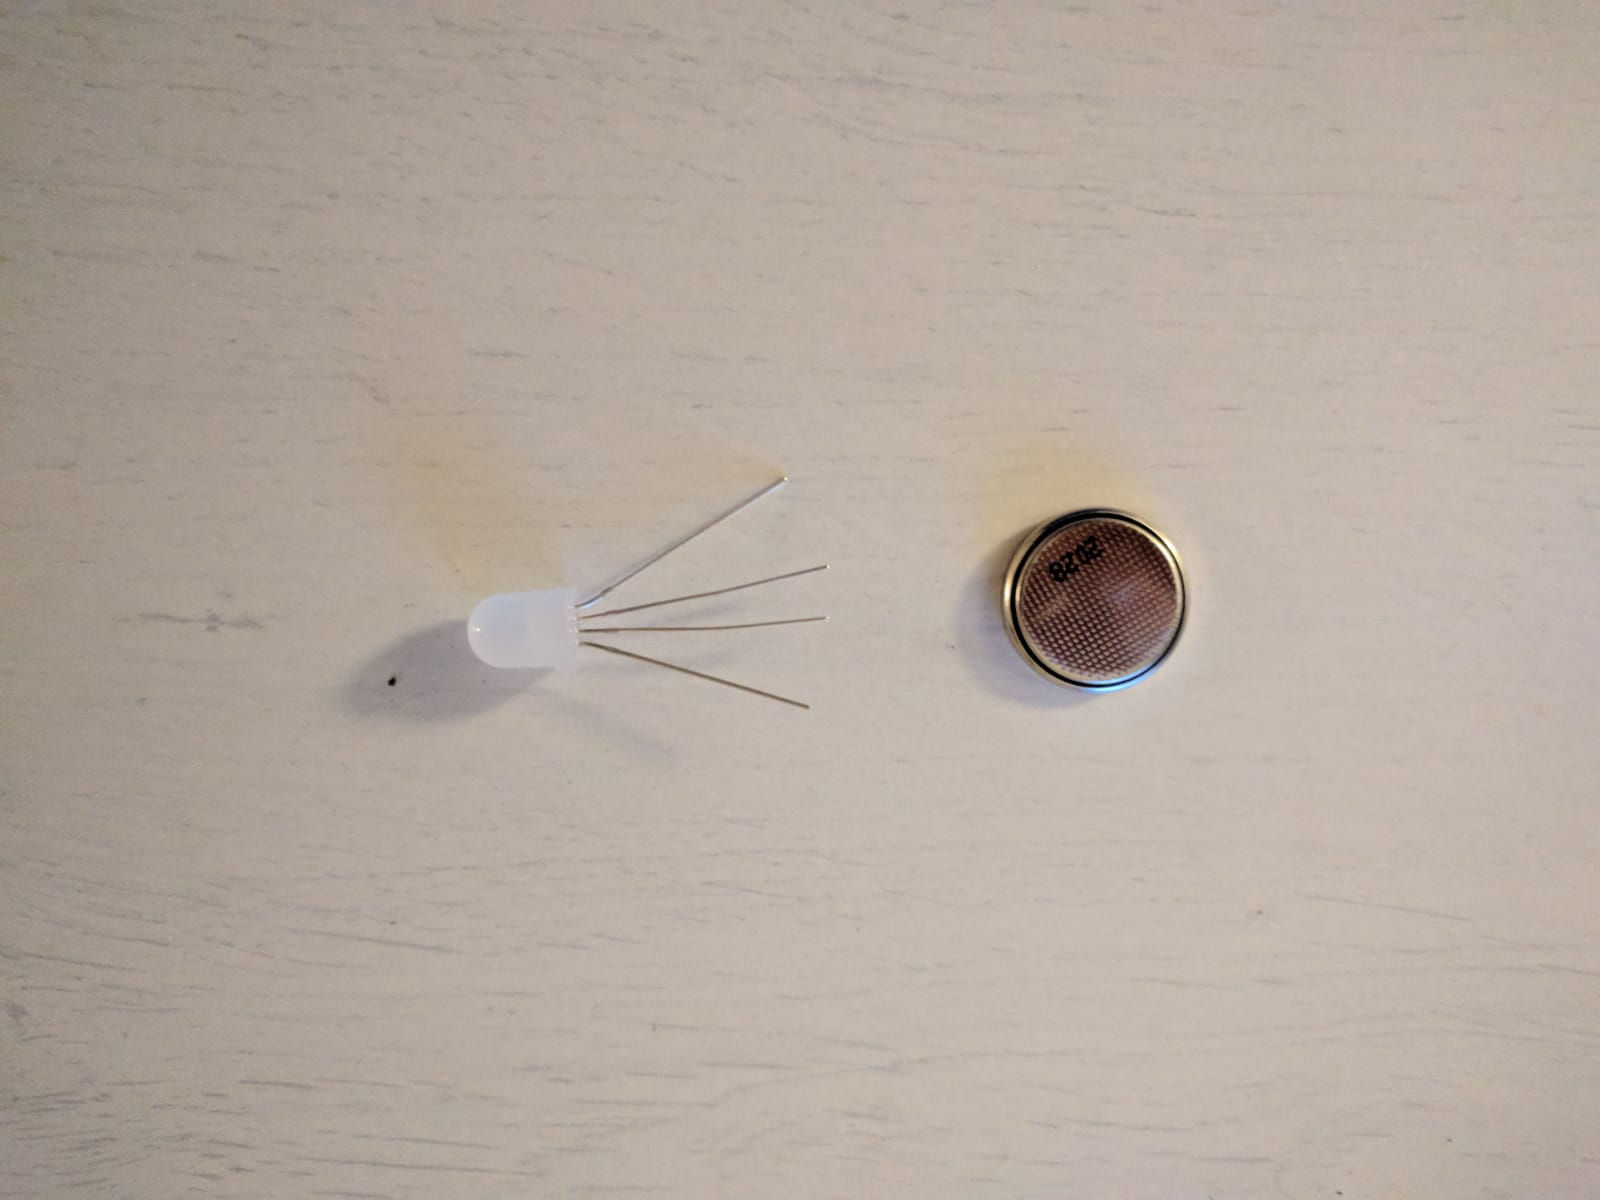
\includegraphics{img/led.jpeg}
  \caption{LED RGB (sinistra) e batteria al litio da $3\:V$ (destra).\label{fig:led}}
\end{figure}

\begin{figure}[H]
  \centering
  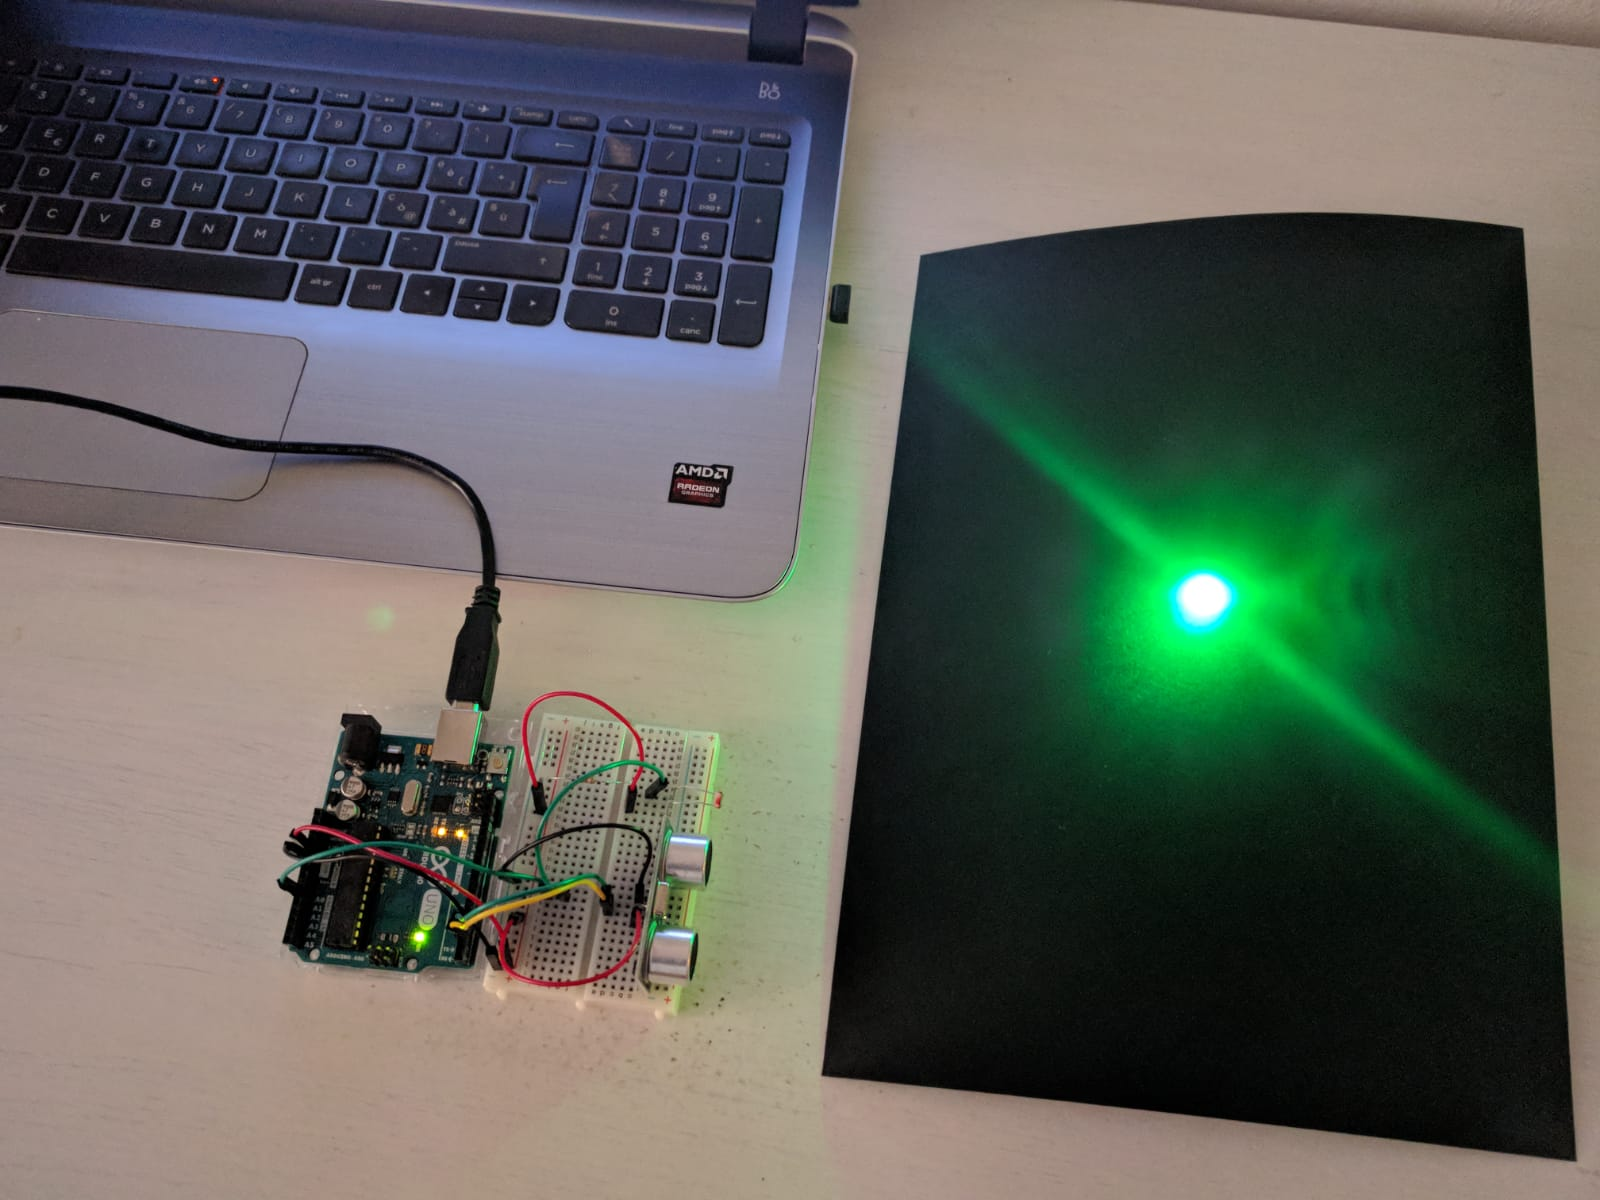
\includegraphics{img/setup.jpeg}
  \caption{Il setup sperimentale.\label{fig:setup}}
\end{figure}

\hypertarget{schema-del-circuito}{%
\subsection{Schema del circuito}\label{schema-del-circuito}}

\begin{figure}[H]
  \centering
  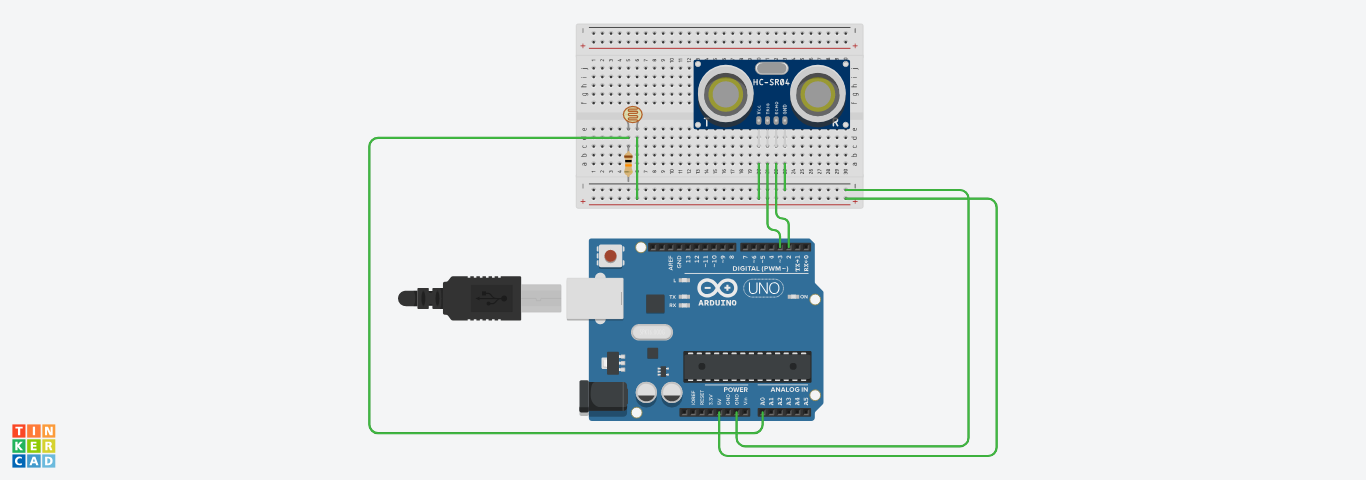
\includegraphics{img/schema.png}
  \caption{Schema del circuito.\label{fig:schema}}
\end{figure}

\hypertarget{sensore-di-luminosituxe0}{%
\subsection{Sensore di luminosità}\label{sensore-di-luminosituxe0}}

La luminosità, a cui è sensibile la fotoresistenza \(R_x\), viene
determinata dalla lettura del potenziale \(V\) fra la fotoresistenza ed
un resistore \(R\) da \(10\:k\Omega\) in serie. Uguagliando le correnti
che attraversano \(R\) ed \(R_x\) abbiamo
\[\frac{V}{R}=\frac{\varepsilon-V}{R_x},\] dove \(\varepsilon=5\:V\) è
la tensione fornita al circuito dalla scheda Arduino UNO. Ne segue che
\[R_x\propto \frac{\varepsilon-V}{V}.\] In base alle specifiche della
fotoresistenza si può considerare una proporzionalità inversa fra
intensità luminosa \(I\) e resistenza \(R_x\) della fotocella. Si può
dunque concludere che \[I\propto \frac{V}{\varepsilon-V}.\] La grandezza
misurata sarà quindi l'intensità adimensionale
\[\frac{I}{I_0}=\frac{V}{\varepsilon-V},\] dove \(I_0\) è l'intensità
corrispondente ad una tensione \(V=\frac{1}{2}\varepsilon=2.5\:V\) e il
cui valore non ha particolare interesse ai fini dell'esperimento.

Per quanto riguarda l'incertezza dell'intensità misurata possiamo
assumere un'incertezza unitaria \(\Delta y\) sulla lettura digitale
\(y\) sul pin A0 e propagare l'errore su \(\frac{I}{I_0}\). Considerato
che \(V=cy\) con \(c=\frac{5.0}{1023}\:V\), otteniamo
\[\Delta\left(\frac{I}{I_0}\right)=\frac{d}{d y}\left(\frac{cy}{\varepsilon-cy}\right)\Delta y=\frac{c\varepsilon}{(\varepsilon-V)^2}.\]

\hypertarget{sensore-di-distanza-ad-ultrasuoni}{%
\subsection{Sensore di distanza ad
ultrasuoni}\label{sensore-di-distanza-ad-ultrasuoni}}

In base alle specifiche del sensore HC-SR04 si può considerare
l'incertezza sulle misure di distanza pari a \(\Delta r=0.3\: cm\).

\begin{figure}[H]
  \centering
  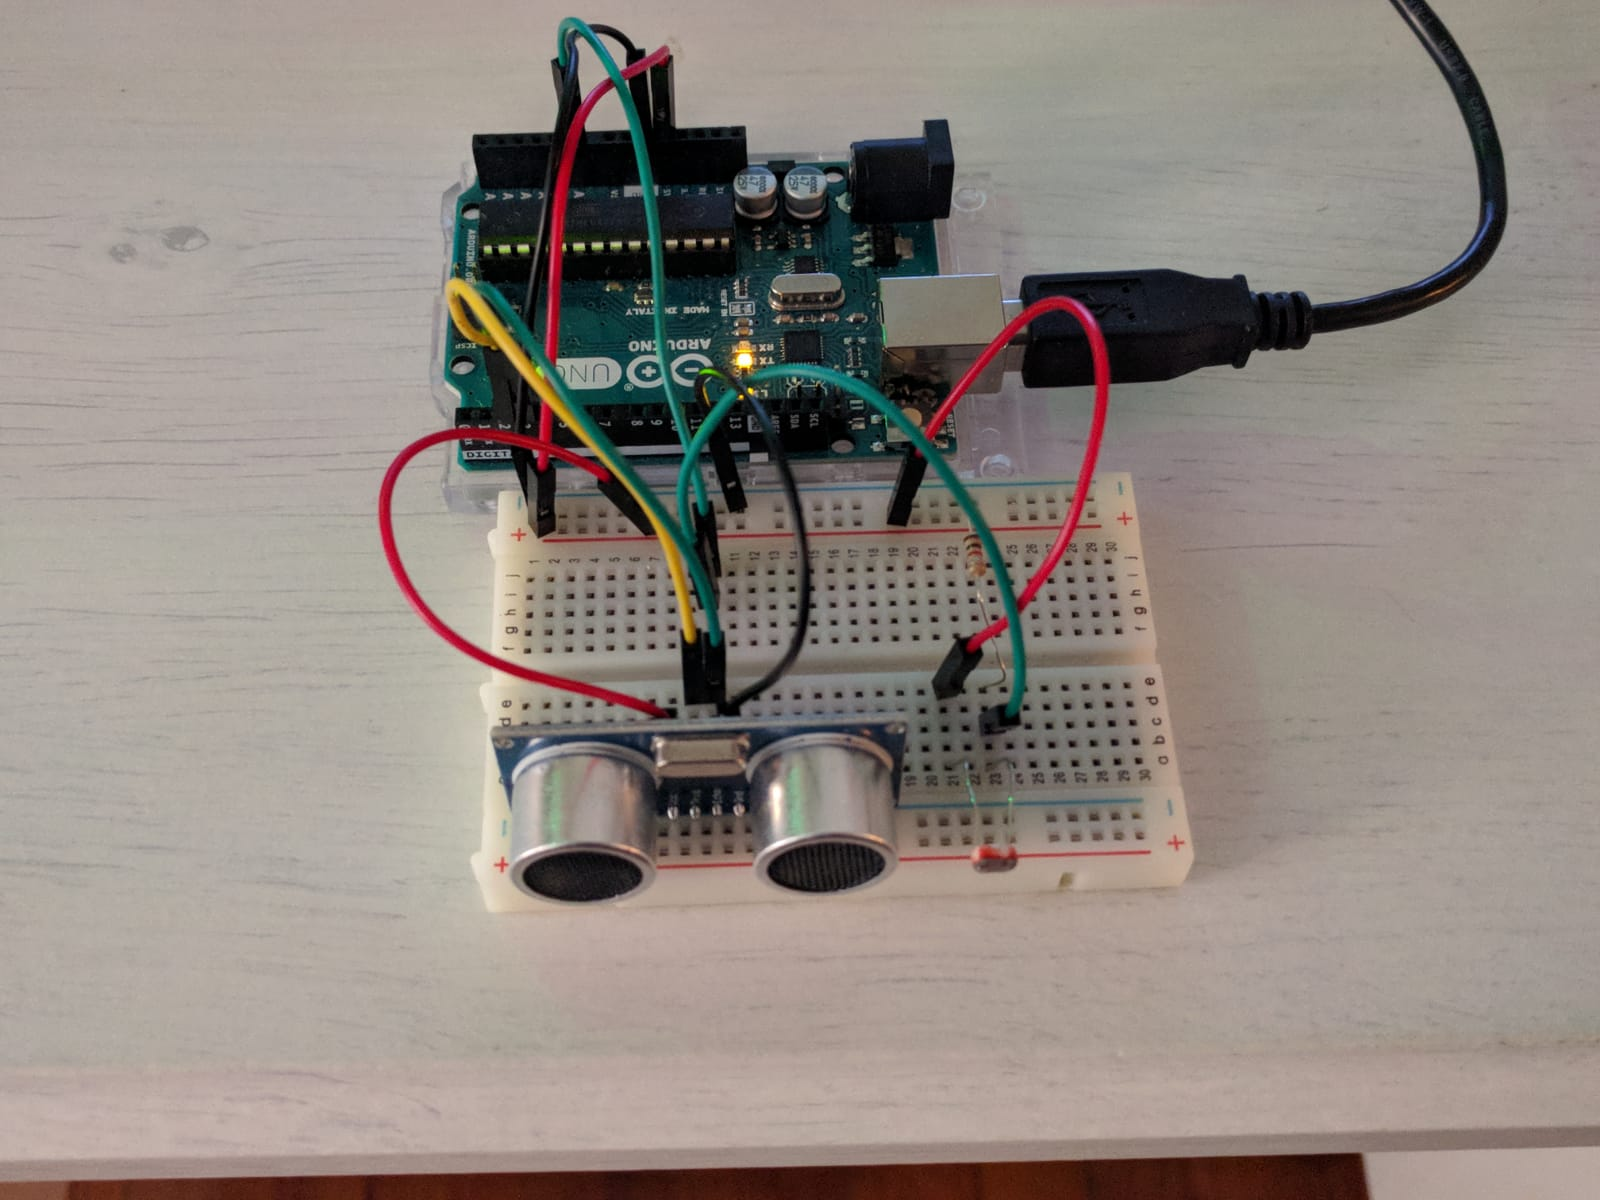
\includegraphics{img/arduino.jpeg}
  \caption{Implementazione del circuito sulla scheda Arduino UNO.\label{fig:arduino}}
\end{figure}

    \hypertarget{codice-arduino}{%
\subsection{Codice arduino}\label{codice-arduino}}

Il codice caricato sull'arduino UNO è il seguente.

\begin{Shaded}
\begin{Highlighting}[]
\DataTypeTok{int}\NormalTok{ photocellPin = A0;}
\DataTypeTok{int}\NormalTok{ triggerPin = }\DecValTok{2}\NormalTok{;}
\DataTypeTok{int}\NormalTok{ echoPin = }\DecValTok{3}\NormalTok{;}

\DataTypeTok{float}\NormalTok{ speedOfSound = }\FloatTok{0.034}\NormalTok{; }\CommentTok{// cm / microseconds}

\DataTypeTok{void}\NormalTok{ setup() \{}
\NormalTok{  pinMode(triggerPin, OUTPUT);}
\NormalTok{  pinMode(echoPin, INPUT);}
\NormalTok{  Serial.begin(}\DecValTok{9600}\NormalTok{);}
\NormalTok{\}}

\DataTypeTok{void}\NormalTok{ loop() \{}
  \DataTypeTok{float}\NormalTok{ t = millis() / }\FloatTok{1000.0}\NormalTok{; }\CommentTok{// secondi dall'avvio del programma}
  \DataTypeTok{int}\NormalTok{ photocellValue = analogRead(photocellPin); }\CommentTok{// lettura della fotoresistenza}
  \DataTypeTok{float}\NormalTok{ V = photocellValue * }\FloatTok{5.0}\NormalTok{ / }\FloatTok{1023.0}\NormalTok{; }\CommentTok{// conversione in tensione}
  \DataTypeTok{float}\NormalTok{ intensity = V / (}\FloatTok{5.0}\NormalTok{ - V); }\CommentTok{// conversione in intensità}
  \DataTypeTok{float}\NormalTok{ intensity_err = }\FloatTok{0.024}\NormalTok{ / ((}\FloatTok{5.0}\NormalTok{ - V) * (}\FloatTok{5.0}\NormalTok{ - V)); \CommentTok{// incertezza}}
\NormalTok{  digitalWrite(triggerPin, LOW);}
\NormalTok{  digitalWrite(triggerPin, HIGH);}
\NormalTok{  delayMicroseconds(}\DecValTok{10}\NormalTok{);}
\NormalTok{  digitalWrite(triggerPin, LOW);}
  \DataTypeTok{float}\NormalTok{ dt = pulseIn(echoPin, HIGH); }\CommentTok{// lettura del tempo di andata e ritorno}
  \DataTypeTok{float}\NormalTok{ distance = speedOfSound * dt / }\DecValTok{2}\NormalTok{; }\CommentTok{// calcolo della distanza}
  \DataTypeTok{float}\NormalTok{ distance_err = }\FloatTok{0.3}\NormalTok{; }\CommentTok{// incertezza}
  \CommentTok{// controlla che il valore sia nel range di sensibilità, quindi stampa le misure }
  \ControlFlowTok{if}\NormalTok{ (distance > }\DecValTok{2}\NormalTok{ && distance < }\DecValTok{400}\NormalTok{) \{ }
\NormalTok{    Serial.print(t);}
\NormalTok{    Serial.print(}\StringTok{" "}\NormalTok{);}
\NormalTok{    Serial.print(distance, }\DecValTok{1}\NormalTok{);}
\NormalTok{    Serial.print(}\StringTok{" "}\NormalTok{);}
\NormalTok{    Serial.print(distance_err, }\DecValTok{1}\NormalTok{);}
\NormalTok{    Serial.print(}\StringTok{" "}\NormalTok{);}
\NormalTok{    Serial.print(intensity, }\DecValTok{4}\NormalTok{);}
\NormalTok{    Serial.print(}\StringTok{" "}\NormalTok{);}
\NormalTok{    Serial.println(intensity_err, }\DecValTok{4}\NormalTok{);}
\NormalTok{  \}}
\NormalTok{  delay(}\DecValTok{300}\NormalTok{);}
\NormalTok{\}}
\end{Highlighting}
\end{Shaded}

    \hypertarget{python}{%
\subsection{Python}\label{python}}

Al fine di analizzare adeguatamente i dati è necessario del software
aggiuntivo. Il linguaggio python consente di interfacciarsi con arduino
attraverso la porta seriale.

\hypertarget{installazione}{%
\subsubsection{Installazione}\label{installazione}}

Il software python si trova alla pagina
\url{https://www.python.org/downloads/} (durante l'installazione spuntare la
voce \texttt{Add\ to\ Path}). Una volta installato python è necessario
installare alcune librerie aggiuntive. Aprire dunque il terminale e
inserire il comando

\begin{Shaded}
\begin{Highlighting}[]
\ExtensionTok{pip}\NormalTok{ install pyserial numpy matplotlib jupyter-notebook}
\end{Highlighting}
\end{Shaded}

\hypertarget{modalituxe0-di-acquisizione-dati}{%
\subsubsection{Modalità di acquisizione
dati}\label{modalituxe0-di-acquisizione-dati}}

I dati possono essere acquisiti in diversi modi:

\begin{itemize}
\item Grafici in tempo reale: eseguire il programma \texttt{plotter.py} attraverso il
comando da terminale (verificare che la porta di arduino sia
\texttt{COM3} o modificare il programma)

\begin{Shaded}
\begin{Highlighting}[]
\ExtensionTok{python}\NormalTok{ plotter.py}
\end{Highlighting}
\end{Shaded}

\item
  Esportazione su foglio di calcolo: eseguire il programma
  \texttt{arduino2excel.py} attraverso il comando da terminale
  (verificare che la porta di arduino sia \texttt{COM3} o modificare opportunamente il
  programma)

\begin{Shaded}
\begin{Highlighting}[]
\ExtensionTok{python}\NormalTok{ arduino2excel.py}
\end{Highlighting}
\end{Shaded}

  L'output del programma è un file in formato \texttt{csv} che può essere importato da \texttt{excel}.

\item
  \href{https://jupyter.org/}{jupyter} notebook: aprire il il notebook \texttt{relazione.ipynb} con il comando da terminale

\begin{Shaded}
\begin{Highlighting}[]
\ExtensionTok{jupyter}\NormalTok{ notebook relazione.ipynb}
\end{Highlighting}
\end{Shaded}

Il codice contenuto nelle celle del notebook può essere eseguito in modalit\'a interattiva
con la combinazione \texttt{Ctrl+Invio} sulla cella selezionata
(per maggiori informazioni su \texttt{jupyter notebook} consultare \url{https://jupyter-notebook.readthedocs.io/en/stable/}).
\end{itemize}

    \hypertarget{acquisizione-dati}{%
\section{Acquisizione dati}\label{acquisizione-dati}}

    Riportiamo una serie di $50$ dati acquisiti.

    \begin{tabularx}{\textwidth}{XXXXX}
\toprule
\# & \(r\) (cm) & \(\Delta r\) (cm) & \(\frac{I}{I_0}\) &
\(\Delta\left(\frac{I}{I_0}\right)\)\\
\midrule
\endhead
0 & 3.1 & 0.3 & 2.9195 & 0.015\\
1 & 3.0 & 0.3 & 2.4915 & 0.0119\\
2 & 3.3 & 0.3 & 2.217 & 0.0101\\
3 & 3.9 & 0.3 & 1.9912 & 0.0087\\
4 & 3.8 & 0.3 & 1.8182 & 0.0078\\
5 & 4.2 & 0.3 & 1.5511 & 0.0064\\
6 & 4.6 & 0.3 & 1.4014 & 0.0056\\
7 & 4.9 & 0.3 & 1.2239 & 0.0048\\
8 & 5.3 & 0.3 & 1.1136 & 0.0044\\
9 & 6.1 & 0.3 & 1.0098 & 0.0039\\
10 & 6.3 & 0.3 & 0.8875 & 0.0035\\
11 & 6.6 & 0.3 & 0.8235 & 0.0033\\
12 & 7.1 & 0.3 & 0.7638 & 0.003\\
13 & 7.9 & 0.3 & 0.7022 & 0.0028\\
14 & 8.0 & 0.3 & 0.6368 & 0.0026\\
15 & 8.4 & 0.3 & 0.586 & 0.0025\\
16 & 9.5 & 0.3 & 0.5246 & 0.0023\\
17 & 10.3 & 0.3 & 0.4614 & 0.0021\\
18 & 10.8 & 0.3 & 0.3995 & 0.0019\\
19 & 12.2 & 0.3 & 0.3496 & 0.0018\\
20 & 13.0 & 0.3 & 0.3048 & 0.0017\\
21 & 14.2 & 0.3 & 0.274 & 0.0016\\
22 & 15.1 & 0.3 & 0.2476 & 0.0015\\
23 & 16.2 & 0.3 & 0.2222 & 0.0015\\
24 & 17.1 & 0.3 & 0.2007 & 0.0014\\
25 & 18.6 & 0.3 & 0.1827 & 0.0014\\
26 & 19.4 & 0.3 & 0.1638 & 0.0013\\
27 & 20.7 & 0.3 & 0.1481 & 0.0013\\
28 & 21.9 & 0.3 & 0.1354 & 0.0013\\
29 & 22.5 & 0.3 & 0.1242 & 0.0012\\
30 & 23.7 & 0.3 & 0.1156 & 0.0012\\
31 & 25.1 & 0.3 & 0.1083 & 0.0012\\
32 & 26.1 & 0.3 & 0.1 & 0.0012\\
33 & 26.6 & 0.3 & 0.0941 & 0.0012\\
34 & 27.3 & 0.3 & 0.0895 & 0.0012\\
35 & 28.1 & 0.3 & 0.086 & 0.0012\\
36 & 29.4 & 0.3 & 0.0803 & 0.0011\\
37 & 28.1 & 0.3 & 0.0837 & 0.0011\\
38 & 26.2 & 0.3 & 0.0965 & 0.0012\\
39 & 24.0 & 0.3 & 0.1095 & 0.0012\\
40 & 22.5 & 0.3 & 0.1205 & 0.0012\\
41 & 21.2 & 0.3 & 0.1341 & 0.0013\\
42 & 19.6 & 0.3 & 0.1533 & 0.0013\\
43 & 17.9 & 0.3 & 0.184 & 0.0014\\
44 & 15.0 & 0.3 & 0.2415 & 0.0015\\
45 & 12.7 & 0.3 & 0.32 & 0.0017\\
46 & 10.4 & 0.3 & 0.413 & 0.002\\
47 & 9.0 & 0.3 & 0.536 & 0.0023\\
48 & 7.0 & 0.3 & 0.7078 & 0.0029\\
49 & 5.7 & 0.3 & 0.9903 & 0.0039\\
\bottomrule
\end{tabularx}

    \hypertarget{analisi-dati}{%
\section{Analisi dati}\label{analisi-dati}}

Riportiamo il grafico distanza-intensit\`a per i dati grezzi (vedi fig.~\ref{fig:data}).

\begin{figure}[H]
  \centering
  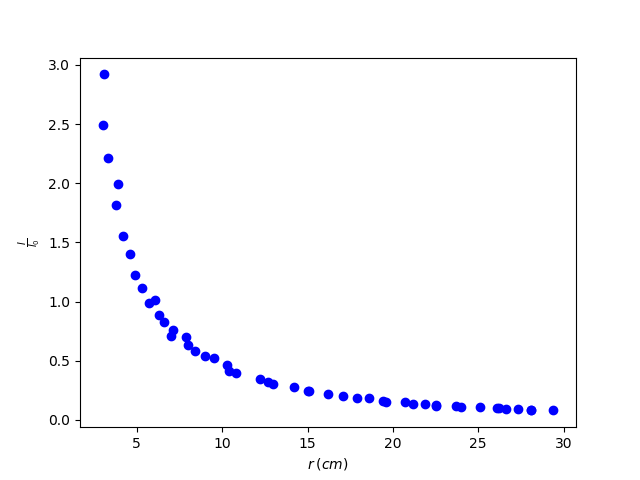
\includegraphics{img/data.png}
  \caption{La relazione distanza-intensit\`a.\label{fig:data}}
\end{figure}

    Verifichiamo ora che \(\frac{1}{r^2}\) e \(I\) siano effettivamente proporzionali.

\begin{figure}[H]
  \centering
  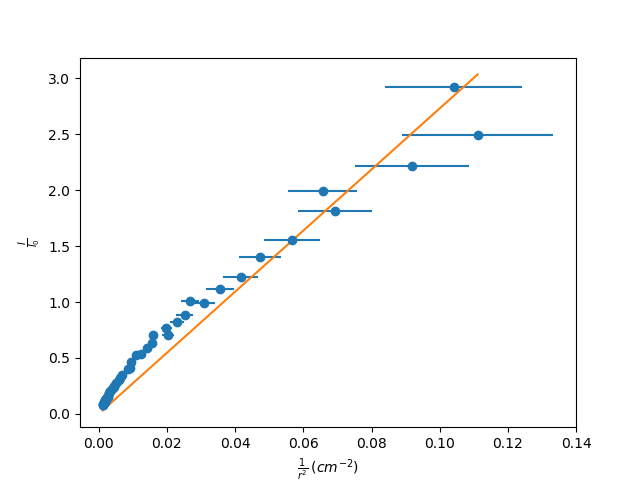
\includegraphics{img/inverse-square-law}
  \caption{La relazione distanza-intensit\'a linearizzata.\label{fig:inverse-square-law}}
\end{figure}

La retta nel grafico di fig.~\ref{fig:inverse-square-law} rappresenta il \emph{best fit}.
Il coefficiente angolare di
tale retta corrisponde a \(\frac{P}{4\pi}\).

    \hypertarget{conclusioni}{%
\section{Conclusioni}\label{conclusioni}}

Come si può osservare dal grafico in fig.~\ref{fig:inverse-square-law}, la legge dell'inverso del
quadrato della distanza può considerarsi adeguatamente verificata entro le incertezze
sperimentali, dominate, specialmente alle piccole distanze, dalla scarsa
sensibilità del sensore HC-SR04. Da sottolineare anche una probabile
sottovalutazione dell'incertezza sulla luminosità determinata dalla
scarsa documentazione della fotocella.

Altre fonti di errore che meriterebbero attenzione sono
\begin{itemize}
  \item il fondo luminoso, difficile da
eliminare totalmente
  \item la precisa relazione luminosit\`a-resistenza delle
fotocelle, non ben documentata nel datasheet della fotoresistenza.
\end{itemize}


    % Add a bibliography block to the postdoc



    \end{document}
